\documentclass{article}

\usepackage{tabularx}

\usepackage{graphicx}
\graphicspath{ {img/} }


\title{RAID Configuration: Pragmatic Selection Strategies}
\author{ARI AG -Marcel Schubert}
\date{30.03.2024}

\begin{document}
\maketitle

\section*{Introduction}
Choosing the right configuration for the logical disks
of your systems is no trivial task. But it is still most of technicians are faced with,
if they have some responsibilities of physical systems. 
\\ \\
The goal of this is to present pragmatic aproaches on
how to choose the right configuration for a specific task at hand. 
It does not show explanation on the deep technical facts.
But can be used to calculate and compare a theoretical basis
to achieve a informed decision or to do further research.
\\ \\
The methology used is simply the analysis of available information online.
Since this is not a scientific report, most information was
not checked beyond plain plausibility. Note that i did not 
create any quantifiably empirical measurements.
\\ \\
The report is divided into three main parts.
In the first part general methods to compare
economical differences are presented.

In the second some methods are shown which can help
calculate the theoretical performance of arrays.
It also includes other factors which can be considered.

In the last part a general checklist is presented which
can be used to quickly tackle the problem of finding an
more or less optimal solution.

\begin{figure}[h]
    \label{fig:raid-overview}
    \caption{Raid Overview \cite{cmu:raidhighperf}}
    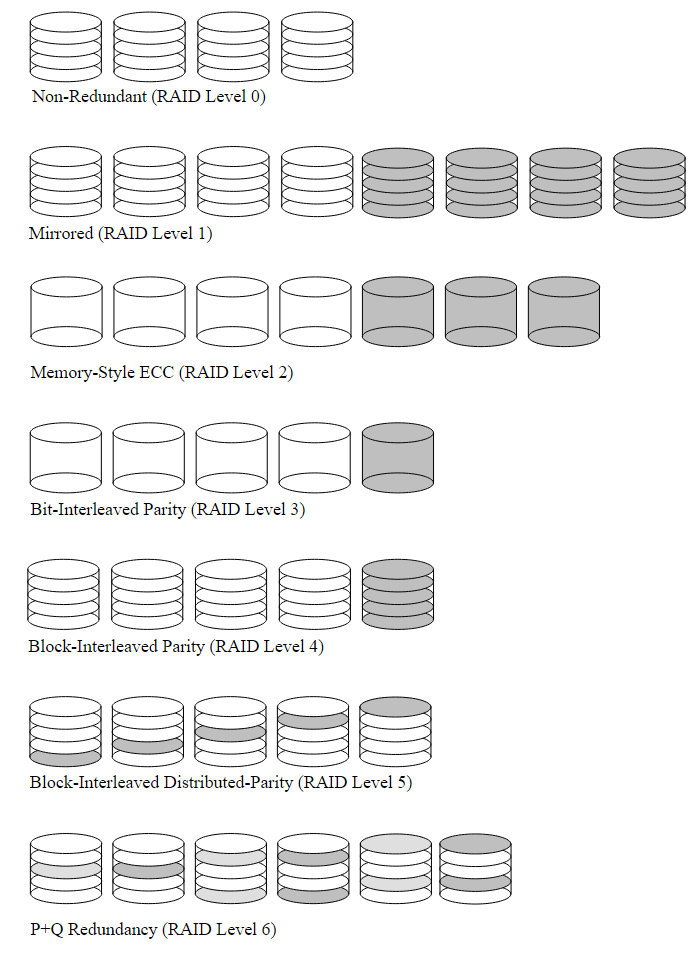
\includegraphics[width=\textwidth]{raid-overview}
\end{figure}

\section{Cost}
Cost can be compared using the matrix shown in Table \ref{tab:economics}.
It is feasable to compare the cost point relative to RAID level-0, since it
is the configuration with the lowest cost/efficiency rating.
To compare the different options use \( N = \textnormal{ Number of disks}\)
and with \(\max\left(x,y\right)\) is the known max function with \( x, y \in R \). \cite{cmu:raidhighperf}

\begin{table}[h]
    \begin{tabularx}{\textwidth}{l|X|X|X|X|X}
        \textbf{Level} &
        Small Read &
        Small Write &
        Large Read &
        Large Write &
        Storage Efficiency \\
        \hline
        0 & 1 & 1 & 1 & 1 & 1 \\
        1 & 1 & \( \frac{1}{2} \) & 1 & \( \frac{1}{2} \) & \( \frac{1}{2} \) \\
        3 & \( \frac{1}{N} \) & \( \frac{1}{N} \) & \( \frac{N-1}{N} \) & \( \frac{N-1}{N} \) & \( \frac{G-1}{N} \) \\
        5 & 1 & \( \max\left(\frac{1}{N},\frac{1}{4}\right) \) & 1 & \( \frac{N-1}{N} \) & \( \frac{N-1}{N} \) \\
        6 & 1 & \( \max\left(\frac{1}{N},\frac{1}{6}\right) \) & 1 & \( \frac{N-2}{N} \) & \( \frac{N-2}{N} \) \\
    \end{tabularx}
    \caption{Throughput Per Dollar Relative to RAID Level-0 \cite{cmu:raidhighperf}}
    \label{tab:economics}
\end{table}

\section{Performance}

\subsection{Other Factors}

\section{Guide}

\section*{Fun Facts}
It appears to be, that RAID was an abreviation for "Redundant Array of Inexpensive Disks" befoire beeing
modified to the more known version of: "Redundant Array of Independent Disks"
Source is: trust me brother, cannot be bothered to look it up.

\bibliographystyle{ieeetr}
\bibliography{refs}

\end{document}